%% Template para Pré-TCC e TCC com base na classe CorujaTeX
%% versão 1.0.0
%% (c) 2021 Colegiado do Curso de Engenharia Elétrica - UFOB
%% 
%% Carrega a classe CorujaTeX
%% Opções: * Tipo do Texto
%%           ptcc  - para proposta de trabalho de conclusão de curso (Pré-TCC)
%%           tcc   - para monografias de graduação - TCC (padrão)
%%           dis   - para dissertações de mestrado
%%         * Paginação
%%           digital  - para impressão em face única (oneside)
%%           impresso - para impressão em frente e verso (twoside) [padrão]
\documentclass[dis,impresso]{CorujaTex}

%\usepackage[grid]{eso-pic, graphicx}
%\usepackage[texcoord,grid,gridunit=mm,gridcolor=black!30,subgridcolor=gray!10]{eso-pic}

%\instituicao{UFOB}
%\brasao{\includegraphics[width=2.61cm]{logo.png}}

%\cidade{Vitória da Conquista-BA}%\department{Colegiado de Eng. Elétrica}

% Curso de graduação
% e.g. \curso{Graduação em Engenharia Elétrica}
% ** Valor padrão: Engenharia Elétrica
%\curso{Engenharia Elétrica}

% Campus
% e.g. \campus{Centro Multidisciplinar de Bom Jesus da Lapa}
% Comente caso não se aplique
\campus{Centro Multidisciplinar de Bom Jesus da Lapa}

% Setor: (Colegiado ou Departamento)
% e.g. \setor{Departamento de Engenharia Elétrica}
% ** Valor padrão: Colegiado de Engenharia Elétrica
\setor{Colegiado de Engenharia Elétrica}

% Título da Monografia/proposta de monografia
% e.g. \titulo{Sistema obtenção do múmero de ranhuras de um MIT}
\titulo{Desenvolvendo uma classe em \LaTeXe}
%\subtitulo{coloque o subtítulo, se houver}

% Autor
% e.g. \author{Thomas Edison}
\autor{Jean-Baptiste Joseph Fourier}

% Orientador(a)
% para orientador do sexo masculino use \orientador{nome}
% e.g. \orientador{Prof. Dr. Nikola Tesla}
% para orientador do sexo feminino use \orientadora{nome}
% e.g. \orientadora{Profa. Dra. Marie Curie}
\orientador{Prof. Dr. Pierre-Simon Laplace}

% Coorientador(a)
% para coorientador do sexo masculino use \coorientador{nome}
% e.g. \coorientador{Prof. Dr. Nikola Tesla}
% para coorientador do sexo feminino use \coorientadora{Nome}
% e.g. \coorientadora{Profa. Dra. Marie Curie}
%\coorientadora{Profa. Dra. Maria Gaetana Agnesi}

% Data da defesa
% e.g. \date{Dezembro de 2012}
\date{Dezembro de 2017}

\begin{document}
	
	%\frontmatter % marca o início da parte pré-textual
	%\pagestyle{empty}
	\printCapa
	
	\printFolhaderosto

	\printfichacatalografica %Insere ficha cat. apenas para OPT=tcc
	
	\printFolhaAprovacao
	
	\printDedicatoria %Insere dedicatória apenas para OPT=tcc
	
	\printAgradecimentos %Insere agradecimentos apenas para OPT=tcc
	
	\printEpigrafe %Insere epígrafe apenas para OPT=tcc 
	
	\printResumo
	
	\printAbstract % insere abstract apenas para OPT=tcc
	
	\printFiguras % lista de figuras
	
	\printTabelas % lista de tabelas
	
	%\listof{quadro}{Lista de Quadros}

	\printQuadros % lista de quadros
	
	\lstlistoflistings % lista de programas
	\thispagestyle{empty}
	
	\printAcronimos % insere lista de abreviaturas, acrônimos e siglas
	
	\printSimbolos % insere lista de Símbolos
	
	\printSumario
	
	%\mainmatter % marca o início da parte textual 
	
	%\newpage
%\pagestyle{empty}

\chapter{INTRODUÇÃO}{}
%\thispagestyle{empty}
%\pagestyle{fancy}
\section{Teste}

Veja no \autoref{qd:Teste} bla bla bla ...

\begin{quadro}[h]
	\centering
	\caption{Estou colocando um quadro no meu texto.}
	%\vspace{5mm}
	\begin{tabular}{|c|c|}
		\hline
		a & b \\
		\hline
		1 & 2 \\
		\hline
	\end{tabular}
	\label{qd:Teste}
\end{quadro}

Observe na \autoref{tab:excel} bla bla bla ...
% Table generated by Excel2LaTeX from sheet 'Planilha1'
\begin{table}[htbp]
	\centering
	\caption{Tabela de teste gerada pela macro Excel2LaTeX}
	\begin{tabular}{rrrr}
		\toprule
		\multicolumn{1}{l}{\textbf{A}} & \multicolumn{1}{l}{\textbf{B}} & \multicolumn{1}{l}{\textbf{C}} & \multicolumn{1}{l}{\textbf{D}} \\
		\midrule
		\rowcolor[rgb]{ .851,  .851,  .851} 1     & 4     & 4     & 16 \\
		2     & 5     & 10    & 100 \\
		\rowcolor[rgb]{ .851,  .851,  .851} 3     & 6     & 18    & 324 \\
		4     & 7     & 28    & 784 \\
		\rowcolor[rgb]{ .851,  .851,  .851} 5     & 8     & 40    & 1600 \\
		6     & 9     & 54    & 2916 \\
		\rowcolor[rgb]{ .851,  .851,  .851} 7     & 10    & 70    & 4900 \\
		\bottomrule
	\end{tabular}%
	\label{tab:excel}%
\end{table}%

% Table generated by Excel2LaTeX from sheet 'Planilha1'
\begin{table}[htbp]
	\centering
	\caption{Add caption}
	\begin{tabular}{m{2cm}|m{2cm}|m{2cm}|m{2.3cm}}
		\toprule
		\multicolumn{4}{c}{\textbf{Dados referentes a nada, apenas para teste}} \\
		\midrule
		\midrule
		\multicolumn{1}{c|}{\textcolor[rgb]{ 1,  0,  0}{\textbf{A}}} & \multicolumn{1}{c|}{\textcolor[rgb]{ 1,  0,  0}{\textbf{B}}} & \multicolumn{1}{c|}{\textcolor[rgb]{ 1,  0,  0}{\textbf{C}}} & \multicolumn{1}{c}{\textcolor[rgb]{ 1,  0,  0}{\textbf{D}}} \\
		\midrule
		\rowcolor[rgb]{ .851,  .851,  .851} 1     & 4     & 4     & R\$ 16,00 \\
		\midrule
		2     & 5     & 10    & R\$ 100,00 \\
		\midrule
		\rowcolor[rgb]{ .851,  .851,  .851} 3     & 6     & 18    & R\$ 324,00 \\
		\midrule
		4     & 7     & 28    & R\$ 784,00 \\
		\midrule
		\rowcolor[rgb]{ .851,  .851,  .851} 5     & 8     & 40    & R\$ 1.600,00 \\
		\midrule
		6     & 9     & 54    & R\$ 2.916,00 \\
		\midrule
		\rowcolor[rgb]{ .851,  .851,  .851} 7     & 10    & 70    & R\$ 4.900,00 \\
		\bottomrule
	\end{tabular}%
	\label{tab:addlabel}%
\end{table}%


% Table generated by Excel2LaTeX from sheet 'Planilha1'
\begin{table}[h]
	\centering
	\caption{Add caption}
	\begin{tabular}{m{2cm}|m{2cm}|m{2cm}|m{2.3cm}}
		\toprule
		\multicolumn{4}{c}{\textbf{Dados referentes a nada, apenas para teste}} \\
		\midrule
		\midrule
		\textcolor[rgb]{ 1,  0,  0}{\textbf{A}} & \textcolor[rgb]{ 1,  0,  0}{\textbf{B}} & \textcolor[rgb]{ 1,  0,  0}{\textbf{C}} & \multicolumn{1}{c}{\textcolor[rgb]{ 1,  0,  0}{\textbf{D}}} \\
		\midrule
		1     & 4     & 4     & R\$ 16,00 \\
		\midrule
		2     & 5     & 10    & R\$ 100,00 \\
		\midrule
		3     & 6     & 18    & R\$ 324,00 \\
		\midrule
		4     & 7     & 28    & R\$ 784,00 \\
		\midrule
		5     & 8     & 40    & R\$ 1.600,00 \\
		\midrule
		6     & 9     & 54    & R\$ 2.916,00 \\
		\midrule
		7     & 10    & 70    & R\$ 4.900,00 \\
		\bottomrule
		\bottomrule
	\end{tabular}%
	\label{tab:addlabel}%
\end{table}%



O progresso tecnológico no mundo teve como marco inicial a descoberta da eletricidade. Diante de uma evolução tão importante, a humanidade pode experimentar um período de grandes descobertas. 
Os motores elétricos têm uma contribuição muito importante para o desenvolvimento da sociedade, seja economicamente e socialmente, fortalecendo o crescimento e evolução das indústrias.
Os primeiros motores foram desenvolvidos pela empresa alemã \textit{Siemens}, que funcionava através da corrente contínua. Tempos mais tarde após a descoberta da corrente alternada os motores de indução trifásicos foram construídos. Os motores de corrente alternada possuem algumas vantagens se comparados aos motores de corrente contínua como simplicidade, baixo custo e máxima eficácia com baixa manutenção. Quanto à classificação, os motores de indução podem ser síncronos, onde a velocidade de rotação é sincronizada com a frequência da rede de alimentação e os motores assíncronos, cuja a velocidade é próxima da velocidade síncrona \cite{Kosow1993}. 

A Equação \eqref{eq:01} descreve o sistema modelado... blá...blá blá 

\begin{equation}
	\label{eq:01}
	\dfrac{10}{s^{2}} 
\end{equation}

\begin{equation}
	%\nonumber
	{X}[{{z}}_k]=\sum^{N-1}_{{n=0}}{{x}[{n}]{(r_0e^{i{\theta }_0})}^{-n}{(R_0e^{i{\varphi }_0})}^{-nk}}, ~~ k=0,1,2,\dots ,M-1 \textrm{}
	%\tag{\ref{eq:19}}
\end{equation}

Nas aplicações industriais, os motores de indução trifásicos (MIT) são predominantes, e como resultados, são destinados ao acionamento de uma grande variedade de cargas. A observação de funcionamento dessas máquinas em condições reais de operação é fundamental para obter informações de demanda de corrente, potência, aquecimento, eficiência e entre outros.

Uma alternativa para obter informações reais de funcionamento de um motor de indução é a criação de um dispositivo que proporcione em laboratório simulações de cargas com diversos  perfis.  As simulações de cargas reais proporcionadas ao motor de indução podem ser impostas por meio de um dispositivo de frenagem com controle eletrônico, sendo capaz de proporcionar  variações de cargas  prédefinidas. Para promover o controle de força de frenagem, a utilização de um dispositivo de fricção como alternativa  implica na necessidade de materiais de elevada resistência ao desgaste, porém  a utilização de um freio por correntes induzidas dispensa essa necessidade, já que a força exercida para a frenagem é proporcionada pelo campo magnético gerado pelas bobinas. O freio eletromagnético por correntes induzidas tem seu princípio de funcionamento o campo magnético gerado pelas bobinas atuando sobre um disco fixado ao motor, desta forma ao variar a potência entregue às bobinas é possível obter uma resposta de frenagem variável \cite{Nolasco2013}. 
Para as simulações de cargas, a utilização de um sistema embarcado  permite  automatizar  diferentes perfis de cargas aplicados ao motor de indução, desta forma, a criação de situações de operações próximas do real funcionamento em campo  torna os ensaios mais significativos. 


Este trabalho irá discutir o desenvolvimento de uma bancada didática para simulação de carga em motores elétricos de indução. O sistema funciona com base em um freio eletromagnético para acoplamento ao motor e uma unidade de controle responsável por simular diversos tipos de cargas mecânicas. O conhecimento de como estes motores se comportam em campo é alvo de bastante estudos e de extrema importância para os trabalhos realizados na matéria de Máquinas Elétricas oferecidas em faculdades de Engenharia Elétrica. Realizar experimentos em motores de indução  nos seus locais de operação nem sempre é possível devido ao risco de acidentes e em alguns casos o ambiente é insalubre.  Os laboratórios para ensaios e simulações de cargas aplicados em motores equipado com o simulador de carga para o motor de indução, permitirá as pessoas interessadas no assunto, maiores conhecimentos didáticos nas realizações de estudos e experiências práticas.


\section{Considerações Iniciais}

Os motores de indução são considerados elementos indispensáveis na maioria dos setores industriais. Para observar o comportamento do motor durante o seu funcionamento, sabendo que nem sempre é possível ter acesso ao seu local de operação, uma alternativa é executar ensaios e simulações de cargas em laboratórios.  

É comum a utilização de um Gerador de corrente contínua (CC) funcionando como carga para motores de indução. Os ensaios realizados nos motores de indução em laboratórios são feitos principalmente através de acoplamento do motor de indução trifásico (MIT) a um Gerador CC. Este sistema apresenta alguns problemas durante o seu funcionamento em rotações baixas, pois o gerador não consegue manter uma corrente constante para suas resistências que estão funcionando como carga \cite{Denardi2013}. Outra observação importante a ser feita é que o preço dos Geradores CC são elevados. Para resolver problemas como estes, o projeto proposto é desenvolvido utilizando um freio eletromagnético que tem seu princípio de funcionamento através das correntes de \textit{Foucault}. O protótipo de uma bancada didática para montagem do projeto é descrita de forma detalhada através de imagens criadas em \textit{software} 3D, permitindo a quem interessar a realização de sua montagem. Todas as informações necessárias para replicar o simulador de carga para motor de indução estão disponíveis neste trabalho. A construção dos circuitos eletrônicos e montagem do freio eletromagnético estão detalhadas nos apêndices.

Para executar as simulações de cargas, foi desenvolvido uma Unidade de Controle onde o usuário poderá determinar diferentes tipos de cargas para os experimentos do motor de indução. Os parâmetros de configurações podem ser observados através de um \textit{display} e alterados com os botões conforme a necessidade do usuário.
 

\section{Organização da monografia}

\begin{description}
	\item[Capítulo \ref{cap:02} --] É descrito os objetivos deste trabalho, bem como a apresentação do problema e sua justificativa. É realizada, também, a contextualização e considerações iniciais.
	
	\item[Capítulo \ref{cap:03} --] É apresentada a fundamentação teórica com alguns conceitos sobre a conversão eletromagnética, funcionamento de motores de indução e freios por correntes induzidas. A apresentação sobre sistemas embutidos também é apresentado neste capítulo.
	
	\item[Capítulo \ref{cap:04} --] A descrição do projeto é feito neste capítulo, apresentando todo o processo de elaboração como: a construção da bancada; montagem dos circuitos eletrônicos de controle; arrumação e montagem do quadro de controle. Também é apresentado neste capítulo o \textit{software} desenvolvido para o funcionamento do simulador.
	
	\item[Capítulo \ref{cap:05} --] São apresentados e discutidos os principais resultados obtidos, bem como propostas para trabalhos futuros.
	
	\item[Capítulo \ref{cap:06} --]  São apresentadas as considerações finais sobre o trabalho.
	
	\item[Referências Bibliográficas --] São apresentadas as referências bibliográficas utilizadas no trabalho.
	
	\item[Apêndice \ref{apendice:01} --] Apêndice contendo o \textit{layout}, esquemático e relação de componentes dos principais circuitos desenvolvidos para o projeto.
	
	\item[Anexo \ref{anexo:01} --] Anexo contendo \textit{datasheets} dos principais circuitos integrados utilizados para o desenvolvimento do projeto.
	
\end{description}

%\newpage
%\thispagestyle{empty}
	\newpage \thispagestyle{empty}
	
	\chapter{CONTEXTUALIZAÇÃO}{}
\label{cap:02}

\section{Considerações Iniciais}
\lipsum %% gera texto apenas para teste

Observe na \autoref{fig:01} a apresentação da marca \corujatex e da UFOB.
\begin{figure}[!h]
	\centering
	\caption{Marcas da UFOB e da Coruja\TeX}
	%\vskip 5mm
	\textbf{\Huge Coruja\TeX} \\
	
\includegraphics[width=2cm]{figuras/logo3}\\
	\autoria{Produzido pelo autor}
	\autoria{\citeonline{Kasper:2014}}
	Fonte: Autoria própria
	%Fonte: \cite{}
	\label{fig:01}
\end{figure}


\section{Algo mais...}


%   \lipsum %% gera texto apenas para teste
O progresso tecnológico no mundo teve como marco inicial a descoberta da eletricidade. Diante de uma evolução tão importante, a humanidade pode experimentar um período de grandes descobertas. 
Os motores elétricos têm uma contribuição muito importante para o desenvolvimento da sociedade, seja economicamente e socialmente, fortalecendo o crescimento e evolução das indústrias. O  .... e o \ac{UFOB} ...\ac{UFOB} \ac{AC} e ... \acp{MIT}

\begin{figure}[!h]
	\centering
	\caption{Teste com tikz para geração de elementos gráficos básicos.}
	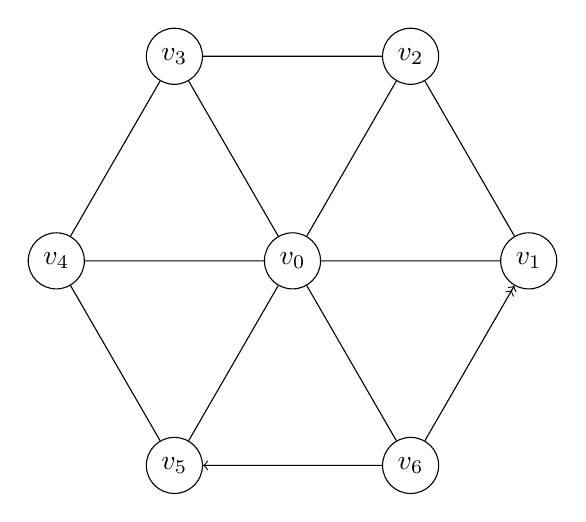
\begin{tikzpicture}
		\tikzstyle{every node}=[draw,shape=circle];
		\node (v0) at (0:0) {$v_0$};
		\node (v1) at ( 0:3) {$v_1$};
		\node (v2) at ( 60:3) {$v_2$};
		\node (v3) at (2*60:3) {$v_3$};
		\node (v4) at (3*60:3) {$v_4$};
		\node (v5) at (4*60:3) {$v_5$};
		\node (v6) at (5*60:3) {$v_6$};
		\draw 
		(v0) -- (v1)
		(v0) -- (v2)
		(v0) -- (v3)
		(v0) -- (v4)
		(v0) -- (v5)
		(v0) -- (v6)
		(v2) -- (v1)
		(v3) -- (v2)
		(v4) -- (v3)
		(v5) -- (v4)
		(v6)[->] -- (v5);
		
		\draw (v1)[<<-] -- (v6);
	\end{tikzpicture}\\
	%\textcolor{black}{Fonte: Carvalho Neto (2017)}%%\citeonline{eumesmo2017}
	\autoria{Autoria própria}
	\label{fig:}
\end{figure}


\begin{center}
	$\dfrac{\omega_s}{\omega_p}$\\ 
	\vspace{5mm}
	$\frac{\omega_s}{\omega_p}$
\end{center}



\begin{equation}
	\centering
	\dfrac{\omega_s}{\omega_p} 
	\frac{\omega_s}{\omega_p}
	\label{eq:teste}
\end{equation}

Os primeiros motores foram desenvolvidos pela empresa alemã \textit{Siemens}, que funcionava através da corrente continua. Tempos mais tarde após a descoberta da corrente alternada os motores de indução trifásica foram construídos.
Os motores de indução podem ser classificados em dois tipos: motores síncronos e assíncronos, onde o motor síncrono de corrente alternada tem como estator, eletroímãs, no qual movimenta em sincronia com a frequência da rede, que no caso do Brasil é 60 HZ, ou seja, variando a frequência da rede, varia-se proporcionalmente a velocidade do motor. Para os motores assíncronos, o mais utilizado, que corresponde a 90\% do mercado, são mais simples, consequentemente mais baratos, também é conhecido como motor de gaiola.
Para manipulação deste tipo de equipamento é importante conhecer informações como: Torque, velocidade e escorregamento, que está relacionado diretamente com as suas características de funcionamento, ou seja, a alteração de qualquer parâmetro acima citado seja através da sua fonte de alimentação, características do motor e/ou carga aplicada, pode determinar a sua forma de operação, sendo ela, eficiente ou ineficiente.
A velocidade de um motor de indução pode ser alterada durante o seu funcionamento normal de trabalho. A carga aplicada ao motor pode determinar mudanças de seu comportamento durante sua operação, sendo assim, um freio eletromagnético acoplado ao motor de indução pode proporcionar ensaios e simulações didáticas através de controles realizados pelo usuário. 

\begin{table}[!h]
	\centering
	\caption[Teste]{Valores aleatórios sem significados.}
	%\vskip 3mm
	\begin{tabular}{c|c|c|c}
		\hline
		A & B & C & D \\
		\hline
		10,00 & 54 & 54 & 74 \\
		\hline
		101,01 & R\$ 21,00 & 41 & 67 \\
		\hline
		74,03 & 85 & 96 & 21 \\
		\hline
		48,00 & 68 & 67 & 58 \\
		\hline
	\end{tabular}
	\vskip 3mm
	Fonte: Autoria própria (2021)
	\label{tab:teste}
\end{table}

Segundo \citeonline{Liu:2011} o freio eletromagnético  por correntes induzidas é desenvolvido por Wouterse em 1991, este estudo descreve que a influência do campo magnético gerado pelas correntes sobre a força de frenagem é em função da velocidade de rotação do disco \cite{Kasper:2014}.
O perfeito acoplamento do freio eletromagnético ao motor de indução proporcionará através de um controle a possibilidade de simulações de cargas, realizado através de um sistema embarcado.

Os microcontroladores, componentes essenciais nos sistemas embarcados, permitem a conexão com dispositivos analógicos e digitais, e através de circuitos simples é possível monitorar e controlar: umidade, luminosidade, velocidade, variação de campo magnético, temperatura, ou seja, infinitas possibilidades.

Diante da importância em simulação de carga para motores de indução, o trabalho proposto terá como desenvolvimento, uma bancada didática para simulação de carga em motores elétricos de indução, bem como a construção de um freio eletromagnético para acoplamento ao motor, e um controle digital para simular diversos tipos de cargas mecânicas. O conhecimento de como estes motores se comportam em campo é alvo de bastante estudos e de extrema importância para os trabalhos realizados na matéria de Maquinas Elétricas oferecidas em faculdades de Engenharia Elétrica. Os laboratórios para ensaios e simulações de cargas aplicados em motores de indução equipado com o simulador de carga para o motor de indução permitirá ao aluno maiores conhecimentos didáticos na realização de estudos e experiências práticas \cite{Liu:2011}.

\begin{citacaodireta}
	As citações diretas, no texto, com mais de três linhas, devem ser
	destacadas com recuo de 4 cm da margem esquerda, com letra menor que a do texto
	utilizado e sem as aspas. Na classe \textbf{\corujatex} recomenda-se a utilização do ambiente \textbf{citacaodireta} \cite[Pg.3]{Liu:2011}.
\end{citacaodireta}

Segundo \citeonline{Liu:2011} os microcontroladores, componentes essenciais nos sistemas embarcados, permitem a conexão com dispositivos analógicos e digitais, e através de circuitos simples é possível monitorar e controlar: umidade, luminosidade, velocidade, variação de campo magnético, temperatura, ou seja, infinitas possibilidades.
Diante da importância em simulação de carga para motores de indução, o trabalho proposto terá como desenvolvimento, uma bancada didática para simulação de carga em motores elétricos de indução, bem como a construção de um freio eletromagnético para acoplamento ao motor, e um controle digital para simular diversos tipos de cargas mecânicas. O conhecimento de como estes motores se comportam em campo é alvo de bastante estudos e de extrema importância para os trabalhos realizados na matéria de Maquinas Elétricas oferecidas em faculdades de Engenharia Elétrica. Os laboratórios para ensaios e simulações de cargas aplicados em motores de indução equipado com o simulador de carga para o motor de indução permitirá ao aluno maiores conhecimentos didáticos na realização de estudos e experiências práticas \cite{Liu:2011}.

Os microcontroladores, componentes essenciais nos sistemas embarcados, permitem a conexão com dispositivos analógicos e digitais, e através de circuitos simples é possível monitorar e controlar: umidade, luminosidade, velocidade, variação de campo magnético, temperatura, ou seja, infinitas possibilidades.
Diante da importância em simulação de carga para motores de indução, o trabalho proposto terá como desenvolvimento, uma bancada didática para simulação de carga em motores elétricos de indução, bem como a construção de um freio eletromagnético para acoplamento ao motor, e um controle digital para simular diversos tipos de cargas mecânicas. O conhecimento de como estes motores se comportam em campo é alvo de bastante estudos e de extrema importância para os trabalhos realizados na matéria de Maquinas Elétricas oferecidas em faculdades de Engenharia Elétrica. Os laboratórios para ensaios e simulações de cargas aplicados em motores de indução equipado com o simulador de carga para o motor de indução permitirá ao aluno maiores conhecimentos didáticos na realização de estudos e experiências práticas \cite{Liu:2011}.

Os microcontroladores, componentes essenciais nos sistemas embarcados, permitem a conexão com dispositivos analógicos e digitais, e através de circuitos simples é possível monitorar e controlar: umidade, luminosidade, velocidade, variação de campo magnético, temperatura, ou seja, infinitas possibilidades.
Diante da importância em simulação de carga para motores de indução, o trabalho proposto terá como desenvolvimento, uma bancada didática para simulação de carga em motores elétricos de indução, bem como a construção de um freio eletromagnético para acoplamento ao motor, e um controle digital para simular diversos tipos de cargas mecânicas. O conhecimento de como estes motores se comportam em campo é alvo de bastante estudos e de extrema importância para os trabalhos realizados na matéria de Maquinas Elétricas oferecidas em faculdades de Engenharia Elétrica. Os laboratórios para ensaios e simulações de cargas aplicados em motores de indução equipado com o simulador de carga para o motor de indução permitirá ao aluno maiores conhecimentos didáticos na realização de estudos e experiências práticas \cite{Liu:2011}.
	\newpage \thispagestyle{empty}
	
	\chapter{TÍTULO DO CAPÍTULO...}{}
\label{cap:03}

\lipsum

\definecolor{verde}{RGB}{25, 90, 25}
\lstset{
	language=c,
	extendedchars=true, % permite acentos
	basicstyle=\ttfamily\scriptsize, 
	keywordstyle=\color{blue}, 
	stringstyle=\color{purple}, 
	commentstyle=\color{verde}, 
	extendedchars=true, 
	showspaces=false, 
	showstringspaces=false, 
	numbers=left,
	numberstyle=\ttfamily\tiny,
	breaklines=true, 
	backgroundcolor=\color{white},
	breakautoindent=true, 
	captionpos=t, %top caption
	xleftmargin=10.5mm,
	tabsize=3,
	framexleftmargin=9.5mm,
	framexrightmargin=-1.0mm, 
	frame=shadowbox, % 〈none|leftline|topline|bottomline|lines|single|shadowbox〉
	rulesepcolor=\color{gray},
	numberbychapter=false,
	backgroundcolor=\color{white},
	firstnumber=86,
	%frameround=tttt
}
\subsection{Ambiente}

O ambiente \textbf{lstlisting} pode ser utilizado para inserção de trecho de códigos de programas importantes para a compreensão do seu trabalho. Ele foi configurado da classe \corujatex para ser designado como \textbf{Programa}. Um exemplo pode observado no \autoref{prog:01}. Analise também no código \LaTeX o comando 

\begin{lstlisting}[caption= Código teste em Linguagem C, label=prog:01] 
void main() 
{
	char slot;
	//configuracoes basicas - sem acentos
	CMCON=0x07;
	ADCON1=0x0F;
	INTCON.GIE=0;
	TRISB.F0=0;
	PORTB.F0=0;
	InicializaMatriz();
	InicializaTeclado();
	InicializaDisplay();
	while(1)
	{
		PORTB.F0=1;
		Delay_ms(250);
		PORTB.F0=0;
		Delay_ms(250);
	}
}	
\end{lstlisting}

\section{Seção do capítulo}
\lipsum %% gera texto apenas para teste

\begin{lstlisting}[caption= Código teste do MikroC for PIC] 
	void main() 
	{
		char slot;
		//configuracoes basicas - sem acentos
		CMCON=0x07;
		ADCON1=0x0F;
		INTCON.GIE=0;
		TRISB.F0=0;
		PORTB.F0=0;
		InicializaMatriz();
		InicializaTeclado();
		InicializaDisplay();
		while(1)
		{
			PORTB.F0=1;
			Delay_ms(250);
			PORTB.F0=0;
			Delay_ms(250);
		}
	}	
\end{lstlisting}

	\newpage \thispagestyle{empty}
	
	\chapter{TÍTULO DO CAPÍTULO...}{}
\label{cap:04}
\section{Seção do capítulo}
\lipsum %% gera texto apenas para teste

	\newpage \thispagestyle{empty}
	
	\chapter{TÍTULO DO CAPÍTULO...}{}
\label{cap:05}
\section{Seção do capítulo}
\lipsum %% gera texto apenas para teste

	\newpage \thispagestyle{empty}
	
	\chapter{TÍTULO DO CAPÍTULO...}{}
\label{cap:06}
\section{Seção do capítulo}
\lipsum %% gera texto apenas para teste
\lipsum 
	\newpage \thispagestyle{empty}
	
	%\backmatter % marca o início da parte pós-textual
 	%\bibliographystyle{abntex2-alf}
 	\bibliography{___postextual/CorujaTexReferencias}
 	\addcontentsline{toc}{chapter}{REFERÊNCIAS} % lista as referências no sumário
 	\newpage \thispagestyle{empty}
 	
 	\appendix
 	
 	\addcontentsline{toc}{chapter}{Apêndice}
\chapter{ALGORÍTIMO PARA ESTIMAR A VELOCIDADE DO MOTOR}
\label{apendice:01}

\section{Algorítmo da STCZT no Matlab}
\definecolor{verde}{RGB}{25, 90, 25}
\lstset{
		language=Matlab,
		extendedchars=true, % permite acentos
		basicstyle=\ttfamily\scriptsize, 
		keywordstyle=\color{blue}, 
		stringstyle=\color{purple}, 
		commentstyle=\color{verde}, 
		extendedchars=true, 
		showspaces=false, 
		showstringspaces=false, 
		numbers=left,
		numberstyle=\tiny,
		breaklines=true, 
		backgroundcolor=\color{white},
		breakautoindent=true, 
		captionpos=t, %top caption
		xleftmargin=10.5mm,
		tabsize=3,
		framexleftmargin=9.5mm,
		framexrightmargin=-1.0mm, 
		frame=shadowbox, %single
		rulesepcolor=\color{gray},
		%numberbychapter=false % deve ser usado antes do begin{document}..yseu na classe...insere numeração sequencial
}

%\lstset{framexleftmargin=6mm, 
%		frame=shadowbox, %single
%		rulesepcolor=\color{gray},
%		numberbychapter=true
%}


\begin{lstlisting}[caption= Algoritimo CZT no Matlab, label=prog:03]
	clc;
	NP=6*512;
	% fs=10000;
	fs=2*5000;
	Ts=1/fs;
	% dx=dfs10k;
	dados=data(:,3); %buffer_60Hz_125_p;  %_amp250_30Hz_variavel_240_025;
	%dados= dfs10k;  %corrente_fs_5k;
	dados=dados - mean(dados);
	NT=length(dados);
	T=NT*fs^-1;
	dp=50;
	d=dp*NP/100;  %4*128;
	NZ=floor((d-NP+NT)/d);
	s=1;
	% f0=25;
	% f1=f0-7;
	% f2=f0+7;
	m=NP;
	h=hanning(NP);
	fredez=zeros(1,NZ);
	dx=dados;
	t_p=(1:NZ)*(d/fs);
	tic;
	resfft=fs/NP;
	for i=1:NZ
	x=dx(s:s+NP-1).*h; 
	y = fft(x,NP); 
	[val idx]=max(abs(y));
	%f0=(idx)*resfft;
	
	%   f0=28;
	%   f1=f0-5;
	%   f2=f0+5;
	f1=22;
	f2=32;
	
	w=exp(-j*2*pi*(f2-f1)/(m*fs));                          % Set complex ratio
	a=exp(j*2*pi*f1/fs);                                    % Set complex starting point
	z=czt(x,m,w,a);                                         % Compute using CZT function
	abs_z=abs(z);
	[l c]=max(abs_z);
	fredez(i)=f1+(c-1)*((f2-f1)/NP);
	s=s+d;
	end
	
	tempo=toc;
	% hold on;
	% plot(t,fredez,'r');
	% figure;
	% plot(t,fsh,'r');
	% xlabel('Tempo(s)');
	% ylabel('Frequencia');
	% title(['STCZT::: Janela:<',num2str(NP),' pontos> Desclocamento:<',num2str(d),' pontos = ',num2str(100*d/NP),'%>']);
	tmax=60;
	figure;
	subplot(2,1,2);
	plot(t_p,60*fredez,'r');
	axis([0 tmax 1740 1790])
	xlabel('Tempo(s)');
	ylabel('Rotacao (RPM)');
	
	subplot(2,1,1);
	pwm_i=data(:,2);
	pwm_i=pwm_i-mean(pwm_i(1:100));
	cmax=60;
	cmin=0;
	pmax=mean(pwm_i)*2,
	pwm_f=cmin+pwm_i*(cmax/pmax);
	tf=0:Ts:length(pwm_f)*Ts - Ts;
	plot(tf,pwm_f,'b');
	axis([0 tmax -3 45])
	% hold on
	% pulso_f=data(:,1); 
	% pulso_f=pulso_f-mean(pulso_f(1:10));
	% plot(tf, pulso_f,'g');
	xlabel('Tempo(s)');
	ylabel('Carga de frenagem (%)');
	% title(['STCZT::: Janela:<',num2str(NP),' pontos> Desclocamento:<',num2str(d),' pontos = ',num2str(100*d/NP),'%>']);
	% clearvars -except -regexp _p$ % limpa todas vari?veis exceto aquelas que terminem com "_p" -> Adem?rio
	%  
	% grid;
	hold off
	
\end{lstlisting}

\section{Seção do apêndice}
\lipsum %% gera texto apenas para teste	
 	\newpage \thispagestyle{empty}
 	
 	\anexo
 	
 	\addcontentsline{toc}{chapter}{Anexo}
\chapter{Título do anexo}{}
\label{anexo:01}
\section{Seção do anexo}
\lipsum %% gera texto apenas para teste
 	\newpage \thispagestyle{empty}
 	
 	\colophon
\end{document}	



%	\input{filename} imports the commands from filename.tex into the target file; it's equivalent to typing all the commands from filename.tex right into the current file where the \input line is.
%	
%	\include{filename} essentially does a \clearpage before and after \input{filename}, together with some magic to switch to another .aux file, and omits the inclusion at all if you have an \includeonly without the filename in the argument. This is primarily useful when you have a big project on a slow computer; changing one of the include targets won't force you to regenerate the outputs of all the rest.
%	
%\input{Lista_AAS.tex} % inserir lista de abreviaturas, acrônimos e siglas